\section{Introduction}
The algorithms described above were implemented in C++ according to the presented pseudocodes. NetworKit and Koala libraries were used for graph data structures. The source code was added to the Koala-NetworKit  GitHub repository.
\section{Implementation Details}
The algorithms are implemented in the following files of the Koala repository:
\begin{itemize}
\item \texttt{include/flow/MaximumFlow.hpp} - Header for all maximum flow algorithms
\item \texttt{cpp/flow/PushRelabel.cpp} - Push Relabel algorithm
\item \texttt{cpp/flow/MKMFlow.cpp} - Malhotra Kumar Maheshwari algorithm
\item \texttt{cpp/flow/BKFlow.cpp} - Boykov-Kolmogorov algorithm
\item \texttt{test/testMaximumFlow.cpp} - Simple unit tests
\item \texttt{benchmark/benchmarkMaximumFlow.cpp} - Benchmark framework for testing algorithms on graphs provided in DIMACS \cite{dimacs} format
\end{itemize}
\section{Results}

\subsection{Datasets}
For testing, two datasets of graph instances were used. First being a set of real life examples of graphs used in computer vision problems and second dataset consists of synthetically generated graphs.

All benchmarks were conducted on a personal computer equipped with an Intel Core i7-6700HQ processor using the Ubuntu 20.04.6 LTS operating system.

\subsection{Instances from Computer Vision}
The first dataset constists of graph instances used in computer vision such as video segmentation, audio restoration, resolution upscaling and mesh segmentation \cite{vision}. The instances were taken from the Min-Cut/Max-Flow Problem Instances Library from the Technical University of Denmark \cite{dataset}. A comprehensive comparison of different maximum flow algorithms designed specifically for computer vision problems on this dataset can be found here \cite{reviewmaxflow}.

During testing a cutoff of 15 minutes (900 seconds) was set. Time execution of algorithms that failed to terminate in that time are marked with "X".

\begin{table}[H]
\centering
\begin{tabular}{lrr|rrr}
\toprule
\textbf{Dataset} & \textbf{Vertices} & \textbf{Edges} & \textbf{PR} & \textbf{MKM} & \textbf{BK} \\
\midrule
graph3x3 & 2,002 & 47,872 & 0.21 & 1.54 & 0.79 \\
graph5x5 & 2,002 & 139,600 & 1.96 & 2.47 & 47.5 \\
rome99 & 3,353 & 8,870 & 8.16 & 3.51 & 0.04 \\
super\_res-E1 & 10,494 & 62,364 & 21.74 & 22.50 & 0.11 \\
super\_res-E2 & 10,494 & 103,164 & 26.40 & 28.01 & 0.13 \\
super\_res-Paper1 & 10,494 & 62,364 & 23.55 & 21.98 & 0.09 \\
texture-Temp & 14,452 & 239,688 & 1.41 & 64.95 & 12.87 \\
handsmall.segment & 15,522 & 94,334 & 538.07 & 159.76 & 1.21 \\
printed\_graph8 & 16,322 & 289,096 & 376.32 & 368.46 & 1.87 \\
printed\_graph14 & 10,514 & 59,7100 & X & 160.26 & 876.19 \\
printed\_graph31 & 9,986 & 564,928 & X & 135.15 & 749.40 \\
bunny.segment & 97,526 & 730,938 & X & X & 194.71 \\
texture-Cremer & 44,034 & 783,128 & X & X & 554.83 \\
\bottomrule
\end{tabular}
\caption{Benchmarking Results for Maximum Flow Algorithms. Time in seconds.}
\end{table}

\subsection{Random Graphs}

The following dataset was created using the \texttt{washington.c} generator authored by Richard Anderson \cite{washington}. The source code for the generator can be found here \cite{washingtonc}. The generator creates 9 different types of graphs of which the ones listed are used in our dataset:
\begin{itemize}
\item \texttt{Mesh Graph/Square Mesh}: A graph with grid like structure and terminals (sink and source) connected to the nodes in the first and last layer.
\item \texttt{Random Level Graph}: A layered graph with edges between nodes in $i$th and $i+1$th layer.
\item \texttt{Line Graph}: Similar to layered graph but with edges allowed between nodes in the same level and between layers $i$ and $i+k$.
\item \texttt{Matching Graph}: A bipartite graph.
\item \texttt{Dinic Bad Case}: A graph that forces all $|V|-1$ iterations of the main loop in the Dinic (and MKM) algorithm.
\item \texttt{Push Relabel Bad Case}: An empirical bade case for the push relabel algorithm.
\end{itemize}

\begin{table}[H]
\centering
\begin{tabular}{lrr|rrr}
\toprule
\textbf{Dataset} & \textbf{Vertices} & \textbf{Edges} & \textbf{PR} & \textbf{MKM} & \textbf{BK} \\
\midrule
 mesh & 2,502 & 7,450 & 5.30 & 5.73 & 0.18 \\
 mesh & 5,627 & 16,800 & 26.93 & 25.54 & 0.56 \\
 mesh & 15,627 & 46,750 & 395.13 & 607.72 & 3.96 \\
\cmidrule(lr){1-6}
 matching & 602 & 1,800 & 0.40 & 0.04 & 0.01 \\
 matching & 4,002 & 12,000 & 22.28 & 2.89 & 0.02 \\
 matching & 10,002 & 30,000 & 187.4 & 20.56 & 0.06 \\
 \cmidrule(lr){1-6}
 line & 2,002 & 5,940 & 8.26 & 4.20 & 0.16\\
 line & 8,002 & 23,945 & 158.92 & 209.03 & 2.41\\
 line & 14,002 & 41,950 & 412.11 & 870.23 & 6.12 \\
\cmidrule(lr){1-6}
 dinic\_bad & 300 & 597 & 0.01 & 0.55 & 0.01 \\
 dinic\_bad & 1,000 & 1,997 & 0.01 & 21.12 & 0.10 \\
 dinic\_bad & 2,000 & 3,997 & 0.01 & 152.62 & 0.55 \\
 dinic\_bad & 5,000 & 9,997 & 0.01 & X & 1.84  \\
\cmidrule(lr){1-6}
 push\_rel\_bad & 1,803 & 2,401 & 0.17 & 0.37 & 0.12 \\
 push\_rel\_bad & 6,003 & 8,001 & 0.57 & 1.08 & 3.71 \\
 push\_rel\_bad & 21,003 & 28,001 & 5.20 & 54.82 & 22.35 \\
\cmidrule(lr){1-6}
 level & 3,000 & 8,600 & 6.01 & 2.68 & 0.24 \\
 level & 6,000 & 17,400 & 15.06 & 19.54 & 1.60 \\
 level & 9,000 & 26,600 & 153.13 & 73.60 & 7.25 \\
 level & 15,000 & 44,500 & 242.34 & 219.09 & 18.28 \\
  
\bottomrule
\end{tabular}
\caption{Benchmarking Results for Maximum Flow Algorithms. Time in seconds.}
\end{table}

\begin{figure}[htbp]
    \centering
    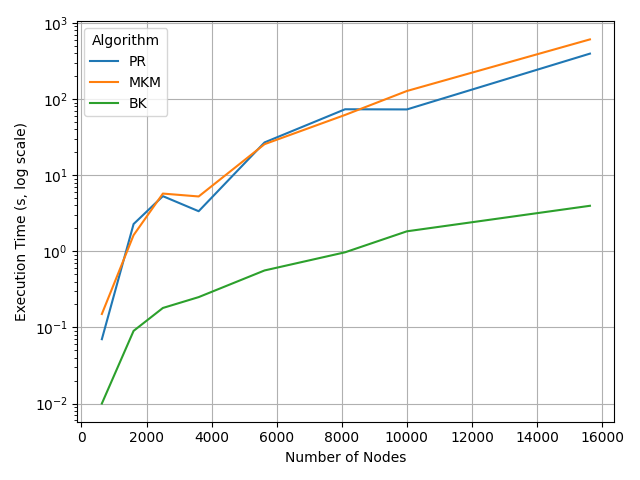
\includegraphics[width=0.8\linewidth]{figures/mesh.png}
    \caption{Mesh instances}
    \label{fig:mesh}
\end{figure}

\begin{figure}[htbp]
    \centering
    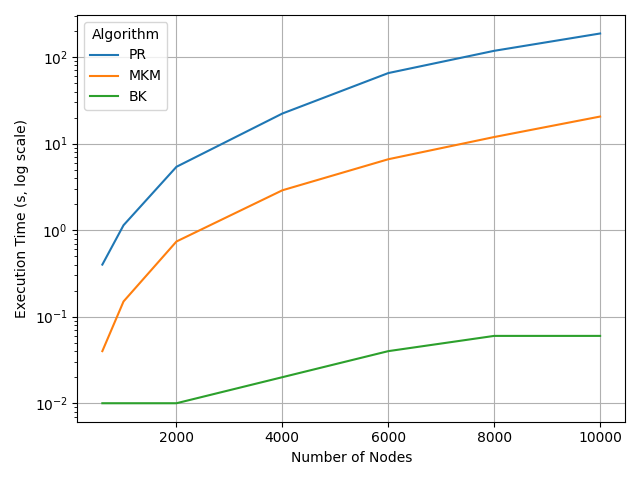
\includegraphics[width=0.8\linewidth]{figures/matching.png}
    \caption{Matching instances with average degree of 4}
    \label{fig:matching}
\end{figure}

\begin{figure}[htbp]
    \centering
    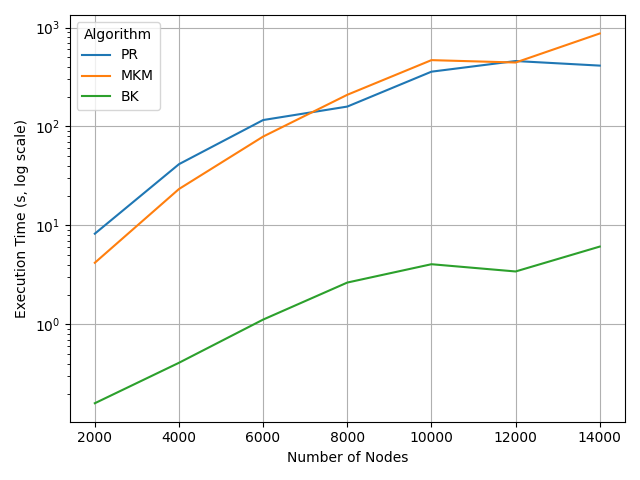
\includegraphics[width=0.8\linewidth]{figures/line.png}
    \caption{Line instances}
    \label{fig:line}
\end{figure}

\begin{figure}[htbp]
    \centering
    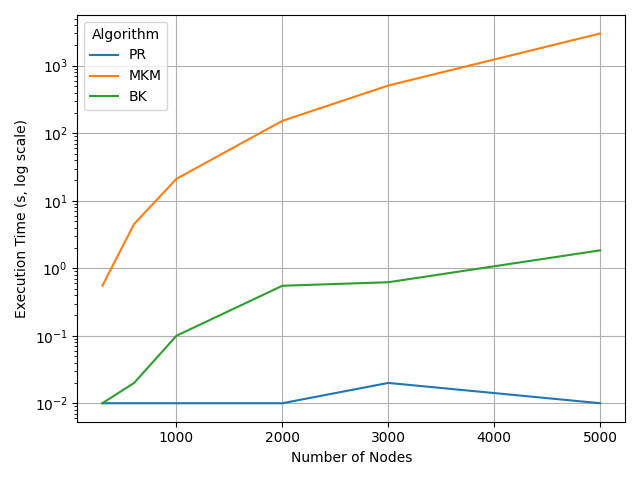
\includegraphics[width=0.8\linewidth]{figures/dinic.png}
    \caption{Bad case for Dinic instances}
    \label{fig:dinic}
\end{figure}

\subsection{Results}

To better understand the empirical time complexity of the three maximum flow algorithms, we performed nonlinear regression to fit models of the form $ t = c \times n^d $, where  $t$  is the execution time and  $n = |V|$  is the number of nodes in the graph. The fitted exponent  $d$  gives insight into how the runtime scales as the input size grows. Table \Cref{tab:complexity_fits} summarizes these results across different graph datasets.

The results indicate that the Boykov-Kolmogorov (BK) algorithm generally exhibits near-quadratic scaling ($ d \approx 1.7 - 2.0 $) on all tested graph types, reflecting superior practical scalability. In contrast, Push-Relabel (PR) and Malhotra-Kumar-Maheshwari (MKM) tend to have higher exponents, often between $2.2$ and $3$, with MKM showing particularly poor scaling (cubic) in challenging cases like the Dinic bad case graph.

\begin{table}[H]
\centering
\small
\begin{tabular}{lccc}
\toprule
\textbf{Dataset} & \textbf{Algorithm} & \textbf{Fitted Model} & \textbf{Interpretation} \\
\midrule
\multirow{3}{*}{Mesh} 
  & PR  & $t \sim n^{2.50}$ & Quadratic scaling, slow \\
  & MKM & $t \sim n^{2.47}$ & Quadratic scaling \\
  & BK  & $t \sim n^{1.78}$ & Sub-quadratic, fastest scaling \\
  
\midrule
\multirow{3}{*}{Line} 
  & PR  & $t \sim n^{2.12}$ & Quadratic scaling \\
  & MKM & $t \sim n^{2.78}$ & Near cubic scaling \\
  & BK  & $t \sim n^{1.93}$ & Near quadratic, better \\
  
\midrule
\multirow{3}{*}{Matching} 
  & PR  & $t \sim n^{2.21}$ & Quadratic scaling \\
  & MKM & $t \sim n^{2.17}$ & Quadratic scaling \\
  & BK  & $t \sim n^{0.73}$ & Nearly linear, very efficient \\
  
\midrule
\multirow{3}{*}{Dinic Bad Case} 
  & PR  & $t \sim n^{0.10}$ & Almost constant \\
  & MKM & $t \sim n^{3.02}$ & Cubic scaling, worst case \\
  & BK  & $t \sim n^{1.95}$ & Near quadratic scaling \\
  
\bottomrule
\end{tabular}
\caption{Fitted empirical complexity models of the form $t = c \times n^{d}$ for execution time $t$ vs. number of nodes $n = |V|$.}
\label{tab:complexity_fits}
\end{table}


The benchmarking results clearly show that the Boykov-Kolmogorov (BK) algorithm consistently outperforms both Push-Relabel (PR) and Malhotra-Kumar-Maheshwari (MKM) algorithms across almost all graph types and sizes. Its runtime remains exceptionally low even as the number of vertices and edges increases, indicating superior scalability and practical efficiency, particularly for structured graphs like mesh (\Cref{fig:mesh}), matching , and line.

Push Relabel generally performs better than MKM algorithm on many datasets, especially in bigger instances. However, it performs poorly on the matching instances graphs (\Cref{fig:matching}). Interestingly, PR performed unexpectedly well on an instance it was theoretically supposed to struggle with. Push Relabel performs more steadily across all graph types, but tends to be slower overall, with particularly high runtimes in large-level and mesh graphs (\Cref{fig:mesh}), making it less suitable for large-scale instances. MKM on the other performs slightly better than PR on small instances (\Cref{fig:line}), but on larger graphs starts to stay behind. Its performance degrades significantly in the Dinic bad case graph (\Cref{fig:dinic}), as expected, due to the nature of the graph forcing the maximum number of iterations in its main loop. 

Overall, these results align well with what is observed in the corresponding performance graphs. BK is the clear winner in practical performance, MKM is effective on small instances but vulnerable to specific worst-case structures, and PR, while robust, lags in speed. This benchmarking underscores the importance of algorithm selection based on input structure in maximum flow applications.